% !TeX root = project-report-cn.tex
% !TeX program = lualatex
% Build: latexmk -lualatex -interaction=nonstopmode -halt-on-error -outdir=.build/project-report-cn project-report-cn.tex
\documentclass[11pt,a4paper,fontset=fandol,scheme=plain]{ctexart}
\usepackage[margin=21mm,headheight=14pt]{geometry}
\usepackage{lmodern,amsmath,amssymb,graphicx,booktabs,array,tabularx}
\usepackage{xcolor,enumitem,fancyhdr,caption,xurl}
\usepackage[colorlinks=true,linkcolor=teal,citecolor=teal,urlcolor=teal]{hyperref}
\definecolor{reportblue}{HTML}{18536B}
\hypersetup{pdftitle={项目报告：神经网络筛选前后的事件选择与质量谱},pdfauthor={HiggsML 项目}}
\pagestyle{fancy}
\fancyhf{}
\fancyhead[L]{\small\textcolor{reportblue}{HiggsML | 项目报告}}
\fancyhead[R]{\small 2026 年 10 月 30 日}
\fancyfoot[C]{\thepage}
\setlength{\parindent}{0pt}
\setlength{\parskip}{6pt}
\setlength{\emergencystretch}{2em}
\setlist[itemize]{leftmargin=1.4em,itemsep=3pt,topsep=4pt}
\captionsetup{font=small,labelfont=bf,justification=raggedright,singlelinecheck=false}
\captionsetup[table]{name=表}
\captionsetup[figure]{name=图}
\newcolumntype{Y}{>{\raggedright\arraybackslash}X}
\newcommand{\reportsection}[1]{\section*{\textcolor{reportblue}{#1}}}
\newcommand{\gev}{\,\mathrm{GeV}}
\newcommand{\status}[1]{\textbf{#1}}
\begin{document}

{\LARGE\bfseries\color{reportblue} 项目报告\par}
\vspace{3pt}
{\Large 神经网络筛选前后的事件选择与质量谱\par}
\vspace{5pt}

\reportsection{1. 项目目标与进展概览}
本项目研究神经网络筛选对四轻子不变质量分布的影响，识别模拟希格斯信号和背景所在的质量区域，
并描述其预期产额与质量谱形状的变化。已完成的比较使用同一最终评估样本，筛选规则均在评估前固定。

\textbf{主要发现。} 两个示例网络均保留了大部分模拟希格斯信号，同时去除了约一半背景产额。
信号仍集中在 125 GeV 附近。背景在筛选前已呈宽广且不均匀的分布；筛选后，剩余背景中位于
信号质量区域的比例上升。因此，背景不仅总量减少，形状也发生变化。这些结论描述的是本项目使用的受控模拟样本。

\begin{table}[h!]
\caption{已完成的比较及其支持材料。}
\label{tab:response}
\small
\begin{tabularx}{\linewidth}{@{}>{\raggedright\arraybackslash}p{.27\linewidth}Y p{.19\linewidth}@{}}
\toprule
分析目标 & 已完成工作 & 支持材料 \\
\midrule
定义筛选前后比较 & 对同一评估总体，比较施加与不施加已冻结高分阈值的结果。 & 第 2、4 章 \\
确定信号区域 & 单独展示信号质量谱，并计算 120--130 GeV 内的产额占比。 & 图~\ref{fig:yields}；表~\ref{tab:fractions} \\
描述背景 & 单独展示实际模拟背景的质量分布。 & 图 1 \\
量化产额与形状变化 & 比较带符号产额的保留率，以及各自归一化的筛选前后谱形。 & 表~\ref{tab:groups}、\ref{tab:yields}、\ref{tab:fractions}；图~\ref{fig:shapes} \\
明确解释边界 & 描述所选事件，并说明统计与物理解释的限制。 & 第 5--7 章 \\
\bottomrule
\end{tabularx}
\end{table}

后文展示两组输入方案在训练随机种子 42 下的比较。A/B/C/D 的具体物理量及组合含义见第二章末，
网络与分数阈值的确定方法见第四章。

项目还持续研究输入变量组对标称信号强度区间宽度 $W_{68}$ 的影响。质量谱为这一比较提供事件选择方面的解释。
第 7 章简述已完成的区间结果；本报告重点说明事件选择与质量谱。

\clearpage
\reportsection{2. 数据与共同物理筛选}
分析使用 ATLAS 2020 教育用途 13 TeV 数据集中的两份模拟样本\cite{OpenData}：
信号 DSID 345060（\texttt{ggH125\_ZZ4lep}）和背景 DSID 363490（\texttt{llll}）。
仅凭背景标签，不能将其认定为纯夸克初态 $ZZ$ 样本。所选末态为 $2e2\mu$，
产额归一化至 $10\,\mathrm{fb}^{-1}$。

\textbf{来源与已有预筛选。} 这两份 MC 文件来自 ATLAS 发布的教育样本；信号文件标记为
125 GeV 的胶子融合希格斯样本，背景为四轻子样本。CERN 记录\cite{OpenData} 的方法说明指出，
该集合在发布前已执行较宽松的对象选择及事件预筛选，保留至少四个轻子（电子或缪子）的事件。
因此，公开 ROOT 条目并非全部未经筛选的生成事件；本项目在此基础上再执行表~\ref{tab:cuts} 的共同筛选。
具体生成器、探测器模拟链和生产级过滤效率，仍需单独的样本生产证据核实。

\begin{table}[h!]
\caption{公开输入与本项目共同筛选后的数量。首行为 ROOT 条目数；其后为 draft001 的物理事件组数，
已核对所选条目与事件组一一对应。后三行是共同筛选总体的互斥划分。}
\label{tab:population}
\centering
\small
\begin{tabular}{lrrr}
\toprule
阶段 & 信号 & 背景 & 合计 \\
\midrule
公开 ROOT 输入（项目筛选前） & 164,716 & 554,279 & 718,995 \\
共同筛选后（全部子集） & 45,083 & 3,593 & 48,676 \\
\quad 训练子集 & 27,026 & 2,175 & 29,201 \\
\quad 验证子集 & 9,008 & 720 & 9,728 \\
\quad 最终评估子集 & 9,049 & 698 & 9,747 \\
\bottomrule
\end{tabular}
\end{table}

上述计数描述公开样本到项目基线的变化，不包含发布前被滤掉的事件，也不构成每条筛选条件的逐步计数。

\textbf{事件结构。} 两份文件的 \texttt{mini} 树具有相同结构，每个条目对应一个事件。
下列为输入配置读取的 19 个分支，顺序与 ROOT 文件一致，已通过文件元数据核对。

\begingroup
\small
\begin{verbatim}
Branch                       ROOT type
runNumber                    int32_t
eventNumber                  int32_t
channelNumber                int32_t
mcWeight                     float
trigE                        bool
trigM                        bool
lep_n                        uint32_t
lep_trigMatched              std::vector<bool>
lep_pt                       std::vector<float>
lep_eta                      std::vector<float>
lep_phi                      std::vector<float>
lep_E                        std::vector<float>
lep_z0                       std::vector<float>
lep_charge                   std::vector<int32_t>
lep_type                     std::vector<uint32_t>
lep_isTightID                std::vector<bool>
lep_ptcone30                 std::vector<float>
lep_etcone20                 std::vector<float>
lep_tracksigd0pvunbiased     std::vector<float>
\end{verbatim}
\endgroup

前七个字段为事件级标量；之后每个向量含 \texttt{lep\_n} 个元素，相同下标对应同一轻子。
\texttt{*Number} 字段标识事件或样本，\texttt{mcWeight} 为带符号生成器权重。
动量、能量和隔离量之和以 MeV 存储，需要时换算为 GeV；\texttt{lep\_z0} 的单位为 mm。
\texttt{lep\_tracksigd0pvunbiased} 存储 $d_0/\sigma(d_0)$。

\textbf{触发条件。} \texttt{trigE} 和 \texttt{trigM} 分别记录电子与缪子触发判定，至少一个须为真。
此外，至少一个通过品质筛选的轻子须满足 \texttt{lep\_trigMatched=true}，将所选轻子与触发判定关联起来。
与文献的详细比较见第 3 章。

\clearpage
\textbf{筛选规则。} 表~\ref{tab:cuts} 先列单分支规则，再列组合条件与重建量条件。
这一分组便于阅读；实际执行顺序见表后说明。

\begin{table}[h!]
\caption{神经网络筛选前的共同筛选，变量采用上列 ROOT 分支名。动量与质量阈值的单位均为 GeV。}
\label{tab:cuts}
\small
\renewcommand{\arraystretch}{1.12}
\begin{tabularx}{\linewidth}{@{}>{\raggedright\arraybackslash}p{.35\linewidth}Y@{}}
\toprule
输入变量 & 项目实际规则 \\
\midrule
\multicolumn{2}{@{}l}{\textbf{单分支规则}} \\
\texttt{lep\_trigMatched} & 四个通过品质筛选的轻子中，至少一个与触发匹配。 \\
\texttt{lep\_pt} & 四个通过品质筛选的轻子按 $p_T$ 降序排列：
$p_{T,1}\geq20$、$p_{T,2}\geq15$、$p_{T,3}\geq10$、$p_{T,4}\geq7$。 \\
\texttt{lep\_type} & 保留电子和缪子：$|\texttt{lep\_type}|\in\{11,13\}$。 \\
\texttt{lep\_isTightID} & 保留严格鉴别（tight-ID）标志为真的轻子。 \\
\midrule
\multicolumn{2}{@{}l}{\textbf{组合条件与重建量条件}} \\
\texttt{trigE}, \texttt{trigM} & 要求 \texttt{trigE=true} 或 \texttt{trigM=true}。 \\
\texttt{lep\_ptcone30}, \texttt{lep\_pt} & 径迹隔离：每个轻子须满足 $p_T>0$ 且
\texttt{lep\_ptcone30}/\texttt{lep\_pt}$<0.3$。 \\
\texttt{lep\_etcone20}, \texttt{lep\_pt} & 量能器隔离：每个轻子须满足 $p_T>0$ 且
\texttt{lep\_etcone20}/\texttt{lep\_pt}$<0.3$。 \\
\nolinkurl{lep_tracksigd0pvunbiased}, \texttt{lep\_type} & 横向碰撞参数显著度的绝对值：电子 $<5$，缪子 $<3$。 \\
\texttt{lep\_z0}, \texttt{lep\_eta} & 纵向碰撞参数条件：
$|\texttt{lep\_z0}/\cosh(\texttt{lep\_eta})|<0.5$ mm。 \\
\texttt{lep\_n} 与品质筛选掩码 & 品质筛选后须恰好剩余四个轻子；原始 \texttt{lep\_n} 可以大于四。 \\
\texttt{lep\_eta}, \texttt{lep\_type} & 四个轻子均须满足接受度条件：电子 $|\eta|<2.47$，缪子 $|\eta|<2.7$。 \\
\texttt{lep\_charge}, \texttt{lep\_type} & 总电荷为零；恰好两个电子和两个缪子；组成两个互不重叠的同味异号（SFOS）轻子对。 \\
\texttt{lep\_pt}, \texttt{lep\_eta}, \texttt{lep\_phi}, \texttt{lep\_E}，
以及 SFOS 配对 & 重建轻子对质量；每个 SFOS 质量均须 $>5$，且
$50<m_{12}<106$、$12<m_{34}<115$。 \\
四个轻子的四动量 & 总不变质量满足 $105\leq m_{4\ell}<140$。 \\
\bottomrule
\end{tabularx}
\end{table}

\textbf{质量符号。} 文献~\cite{ATLAS13} 中，$m_{12}$ 为质量最接近标称 $Z$ 质量的 SFOS 对的质量，
$m_{34}$ 为剩余一对的质量。它们由轻子四动量重建，在代码中分别记为 \texttt{mZ1} 和 \texttt{mZ2}。
配对编号不表示按 $p_T$ 排序。

\textbf{执行顺序。} 触发检查后，依次执行味道、tight-ID、径迹隔离、量能器隔离和横向、纵向碰撞参数筛选，
每步至少保留四个轻子。随后要求恰好四个合格轻子，再执行触发匹配、按序 $p_T$、接受度、电荷与配对、
轻子对质量及研究总体条件。所有模型使用相同基线：“筛选前”指已通过这些条件，
“筛选后”则仅额外施加已冻结的网络分数阈值。


\textbf{网络输入：A/B/C/D 四组物理量。} 原始轻子分支经共同筛选和重建后，组成下列 19 个输入。
轻子按 $p_T$ 降序编号；$Z_1/Z_2$ 对应上文的 $m_{12}/m_{34}$ 配对。

\begin{table}[h!]
\caption{输入变量分组及其物理含义。动量和质量使用 GeV，方位角使用弧度。}
\label{tab:features}
\small
\renewcommand{\arraystretch}{1.12}
\begin{tabularx}{\linewidth}{@{}p{.05\linewidth}p{.43\linewidth}cY@{}}
\toprule
组 & 代码变量 & 维数 & 物理含义 \\
\midrule
A & \texttt{lep1\_pt}--\texttt{lep4\_pt}；\texttt{lep1\_eta}--\texttt{lep4\_eta} & 8 &
单轻子的横动量和赝快度，描述动量尺度及相对束流的方向。 \\
B & \texttt{mZ1}, \texttt{mZ2}；\texttt{deltaR\_Z1}, \texttt{deltaR\_Z2} & 4 &
两个轻子对的质量，以及各对内部的角分离 $\Delta R=\sqrt{(\Delta\eta)^2+(\Delta\phi)^2}$。 \\
C & \texttt{pt4l}, \texttt{deltaPhi\_ZZ} & 2 &
四轻子系统的横动量，以及两个轻子对之间的方位角差绝对值。 \\
D & \texttt{cos\_theta\_star}, \texttt{cos\_theta\_1}, \texttt{cos\_theta\_2}；
\texttt{phi\_decay\_planes}, \texttt{phi\_production\_plane} & 5 &
一个产生角余弦、两个衰变极角余弦，以及描述衰变平面与产生平面相对取向的两个角。 \\
\bottomrule
\end{tabularx}
\end{table}

ABCD/BCD/ACD/ABD/ABC 分别使用 19/11/15/17/14 维输入，各自独立训练。
D 组角度在相应静止系中定义，采用负轻子和实验室正束流方向的固定约定。
各组共享底层轻子信息、彼此相关；虽不显式输入 $m_{4\ell}$，仍可能包含质量信息。

\clearpage
\reportsection{3. 外部来源支持哪些条件？}
\textbf{已发表的物理分析。} ATLAS 13 TeV 四轻子分析\cite{ATLAS13} 第 5.1--5.2 节，
为轻子接受度、按序横动量、SFOS 配对、主导与次主导 $Z$ 质量窗口，以及电子和缪子的碰撞参数显著度上限
提供了具体参考。$m_{Z2}$ 的 $12\gev$ 下限与该文献对 $m_{4\ell}<140\gev$ 的规定一致，
覆盖本项目的整个质量窗口。这些对应关系支持筛选条件的物理动机，但不意味着本项目复现了该测量。

\textbf{解释筛选时需要说明的差异。}
\begin{itemize}
\item 文献采用宽松电子鉴别和详细的缪子类型要求；本项目对两类轻子统一使用现有 tight-ID 标志。
尚未证实它与已发表工作点等价。
\item 前三个动量尺度 20、15、10 GeV 与文献一致。本项目允许阈值处取等号，并统一采用 7 GeV 的第四轻子阈值。文献要求电子 $E_T>7\gev$、缪子 $p_T>5\gev$，对量能器标记缪子另设更高阈值。
因此，第四轻子条件及统一使用 $p_T$ 属于项目改动。
\item 文献要求径迹隔离低于 15\%，电子量能器隔离低于 20\%、缪子低于 30\%，并规定了详细的锥大小和修正。
本项目对两个存储的隔离量统一采用 30\% 上限，是项目简化，而非该文献的完整隔离规定。
\item 文献允许多个四轻子候选组合，并执行角分离及其他重建程序。本项目要求恰好四个合格轻子，
且仅使用双电子双缪子样本。项目的 5 GeV 条件检查所有 SFOS 对；文献则在 $4e/4\mu$ 道中讨论替代配对否决。
在本项目中，更严格的 $Z$ 质量窗口已约束两个物理 SFOS 对。
\end{itemize}

\textbf{官方教育示例。} 文献~\cite{HZZCuts,HZZAnalysis} 指定版本的 \texttt{HZZCuts.py}
第 2--25 行定义四轻子多重数、总电荷为零、味道，以及第二、第三轻子的 15/10 GeV 阈值。
其隔离函数（第 28--33 行）排除比值大于 0.3 的情况，而本项目要求严格小于 0.3。
尤其需要注意，\texttt{HZZAnalysis.py} 第 162--168 行已注释掉这些隔离函数的调用，
因此不能据此声称该示例执行了本项目的完整隔离筛选。
Run-1 分析\cite{ATLASRun1} 第 5.1 节支持触发匹配原则，但其触发处理更为详细。

\textbf{尚未确认的来源与归一化差异。} 在已核对来源中，tight-ID 选择和
$|z_0\sin\theta|<0.5$ mm 的确切外部出处仍未确认，因此将其报告为项目固定选择。
项目采用生成器权重和固定样本归一化；官方教育示例还乘以堆积、轻子及触发尺度因子
（文献~\cite{HZZAnalysis} 第 140--142 行）。因此，当前权重定义不应被期待复现其公布或示例产额。

\clearpage
\reportsection{4. 神经网络筛选与保留样本}
\textbf{样本分工。} 共同筛选总体按物理事件组，以 60\%、20\%、20\% 的概率分配至训练、验证和最终评估子集，
实际数量见表~\ref{tab:population}。同一物理事件组始终留在同一子集，所有模型和种子使用相同分配。
训练拟合输入标准化和网络参数；验证选择检查点与阈值；最终评估仅应用已冻结的模型与阈值。
这些比例是分配概率，有限样本计数不必恰好为 60/20/20。

\textbf{网络结构与训练。} 每种输入方案使用一个全连接二分类网络，结构为
\[
 d_{\rm in}\longrightarrow64\longrightarrow64\longrightarrow32\longrightarrow1.
\]
三个隐藏层均使用 LayerNorm 和 SiLU 激活，前两个隐藏层后加入概率 0.1 的 Dropout。
输出经 sigmoid 转为 $0$--$1$ 的分数 $s$；训练标签为信号 1、背景 0，较高分数倾向于信号。
该分数用作排序判别量，不将其解释为已校准的物理信号概率。ABCD 与 BCD 的输入维数分别为 19 和 11。

每个输入用训练集均值和标准差标准化，验证、评估沿用相同变换。
损失为加权二元交叉熵，训练权重取物理权重的绝对值，再除以各训练类别的平均绝对权重；
这不强制两类总权重相等。优化器为 AdamW，学习率 $10^{-3}$、权重衰减 $10^{-4}$，批量大小 1024，
采用 CPU float32，最多训练 200 轮。每轮按绝对物理权重计算验证 AUC（ROC 曲线下面积）；
相对已保留最优值提高超过 $10^{-4}$ 才更新检查点，连续 20 轮未更新则提前停止。
种子 42 的 ABCD 在第 87 轮停止、保留第 67 轮；BCD 在第 86 轮停止、保留第 66 轮。

\textbf{分数阈值如何得到？} 恢复所选检查点后，只取\emph{验证集背景}的分数，按从小到大排序。
令 $a_i=|w_i|$ 为其绝对物理权重，依次累计 $a_i$；第一次达到总绝对权重一半的分数就是阈值：
\[
 k=\min\left\{j:\sum_{i=1}^{j}a_{(i)}\geq\frac12\sum_i a_i\right\},
 \qquad t=s_{(k)}.
\]
下标 $(i)$ 表示按分数排序。此处不作分数插值；评估时 $s\geq t$ 为高分类别，$s<t$ 为低分类别，
同分事件整体进入同一类别。

\textbf{教学示例（非实际运行数据）。} 假设五个验证背景事件的有序分数为
$0.10,0.30,0.60,0.80,0.90$，对应绝对权重为 $1,2,1,4,2$。
总权重为 10，一半为 5；累计权重依次为 $1,3,4,8,10$，首次达到 5 的位置对应 $t=0.80$。
因此分数 0.80 和 0.90 进入高分类别，其绝对权重占比为 $6/10=60\%$。
离散权重和同分事件使该比例不必恰好为 50\%，更不要求评估集的\emph{带符号}背景保留率为 50\%。

实际种子 42 的阈值为 ABCD 的 $0.746724$ 和 BCD 的 $0.860891$（展示时舍入，评估使用原始精度）。
阈值在查看评估质量谱前已冻结，各模型分别确定阈值，未按最终评估结果调节。

\clearpage
\textbf{评估子集的事件数与产额。} 以下比较均使用同一最终评估子集。高分子集用于展示筛选效果；
区间推断仍使用高分和低分两个类别，见第 7 章。

\begin{table}[h!]
\caption{最终评估样本中的物理事件组数。后两列为种子 42 的高分子集，并非新的独立样本。}
\label{tab:groups}
\centering
\begin{tabular}{lrrr}
\toprule
过程 & 基线（网络筛选前） & ABCD 高分 & BCD 高分 \\
\midrule
信号 & 9,049 & 8,761 & 8,563 \\
背景 & 698 & 386 & 378 \\
\bottomrule
\end{tabular}
\end{table}

表~\ref{tab:groups} 的基线仅指共同物理筛选后的评估子集；全部所选样本见表~\ref{tab:population}。
例如，ABCD 高分保留了 8,761/9,049 个信号事件组，而下表的信号产额保留率为 96.80\%。
两者不同，因为前者按事件组计数，后者按带符号物理权重计算。

\begin{table}[h!]
\caption{$10\,\mathrm{fb}^{-1}$ 下的预期带符号产额及保留率。
误差为固定网络和阈值下按物理事件组计算的 MC 标准误差；保留率误差包括筛选前后共享事件的协方差。}
\label{tab:yields}
\centering
\begin{tabular}{llrr}
\toprule
过程 & 选择 & 预期产额 & 保留率（\%） \\
\midrule
信号 & 筛选前 & $2.7710\pm0.0293$ & --- \\
 & ABCD 高分 & $2.6824\pm0.0288$ & $96.80\pm0.19$ \\
 & BCD 高分 & $2.6215\pm0.0285$ & $94.60\pm0.24$ \\
背景 & 筛选前 & $2.3553\pm0.1683$ & --- \\
 & ABCD 高分 & $1.2027\pm0.1202$ & $51.06\pm3.57$ \\
 & BCD 高分 & $1.1012\pm0.1156$ & $46.75\pm3.57$ \\
\bottomrule
\end{tabular}
\end{table}

产额是加权物理期望，不是表~\ref{tab:groups} 中的模拟事件组数。评估产额权重为带符号物理权重
除以分配概率 0.2，以估计同一 $10\,\mathrm{fb}^{-1}$ 曝光下的产额。
三个子集不能作为独立亮度相加。负生成器贡献予以保留。

\textbf{筛选小结。} ABCD 去除约 49\% 的背景产额、损失约 3\% 的信号；BCD 去除约 53\% 的背景、
损失约 5\% 的信号。各自固定阈值下，BCD 对两种过程均筛选得更严格。
仅凭这一点不能视为等效率比较，也不能证明某分类器更优。

\clearpage
\reportsection{5. 信号和背景位于哪里？}
图~\ref{fig:yields} 展示神经网络筛选前后的不变质量分布。左列为模拟希格斯信号，右列为背景。
每个面板在相同亮度和质量分箱边界下，比较基线与其高分子集。

\begin{figure}[h!]
\centering
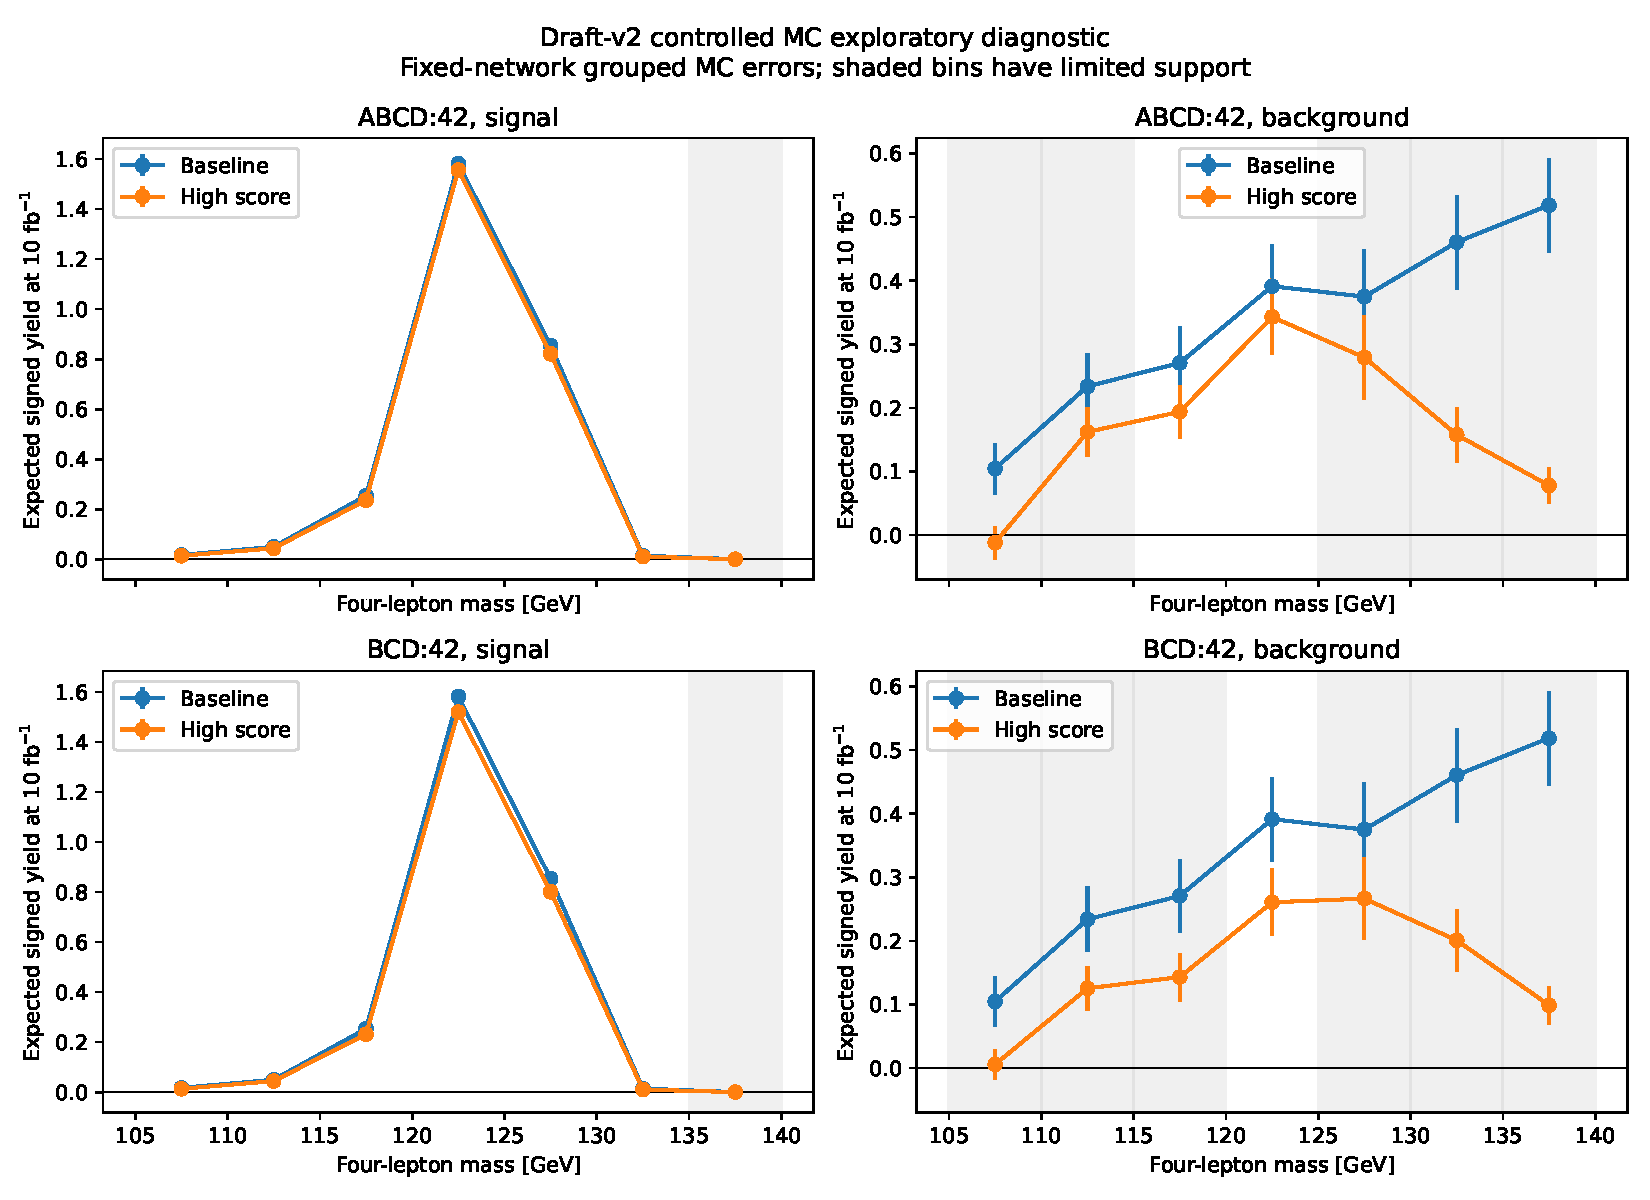
\includegraphics[width=\linewidth]{figures/draft001/mass-yields.pdf}
\caption{draft001 最终评估的带符号质量谱。上排为 ABCD，下排为 BCD，均使用种子 42。
蓝色圆点为基线，橙色菱形为高分事件；左列为信号，右列为背景。每点代表一个 5 GeV 箱，
连线仅作视觉引导，不代表连续质量模型。纵轴为 $10\,\mathrm{fb}^{-1}$ 下的预期产额，信号与背景刻度不同。
误差棒采用按事件组计算的 MC 方差。阴影按下述标准标记统计支持不足的区域；负产额保留。}
\label{fig:yields}
\end{figure}

\textbf{统计支持标记。} 若某质量箱的基线或高分样本满足任一条件，则标为阴影：无事件组；
带符号产额 $Y$ 或分组方差 $V$ 非正；带符号有效计数 $N_{\rm eff}=Y^2/V<20$；
或抵消比 $\rho=|Y|/\sum_i|w_i|<0.2$。其中 $w_i$ 为事件的评估产额权重，
$V$ 为各物理事件组产额贡献的平方和。阴影属于统计支持诊断，并非置信带。
图~\ref{fig:shapes} 的归一化谱形采用相同标准。

\textbf{信号位置。} 模拟信号集中在 125 GeV 附近，两条筛选后曲线基本保留该区域。
网络不改变单个事件的质量；分布变化来自对基线事件的子集选择。粗分箱不能证明峰位移动、
探测器分辨率改善或希格斯物理宽度变化。

\textbf{背景分布。} 背景覆盖整个质量窗口，筛选前已不均匀。不同质量区域的压低程度不同，
高质量尾部尤其明显。因此，信号在视觉上更突出需要从两方面解释：背景减少了多少，以及剩余背景如何分布。
下一页分别归一化的谱形用于回答第二个问题。

\clearpage
\reportsection{6. 谱形如何变化？}
图~\ref{fig:shapes} 将每个过程、每种选择分别除以其自身带符号总产额，从比较中去除总体产额变化。
表~\ref{tab:fractions} 使用固定质量区域量化主要可见变化。

\begin{figure}[h!]
\centering
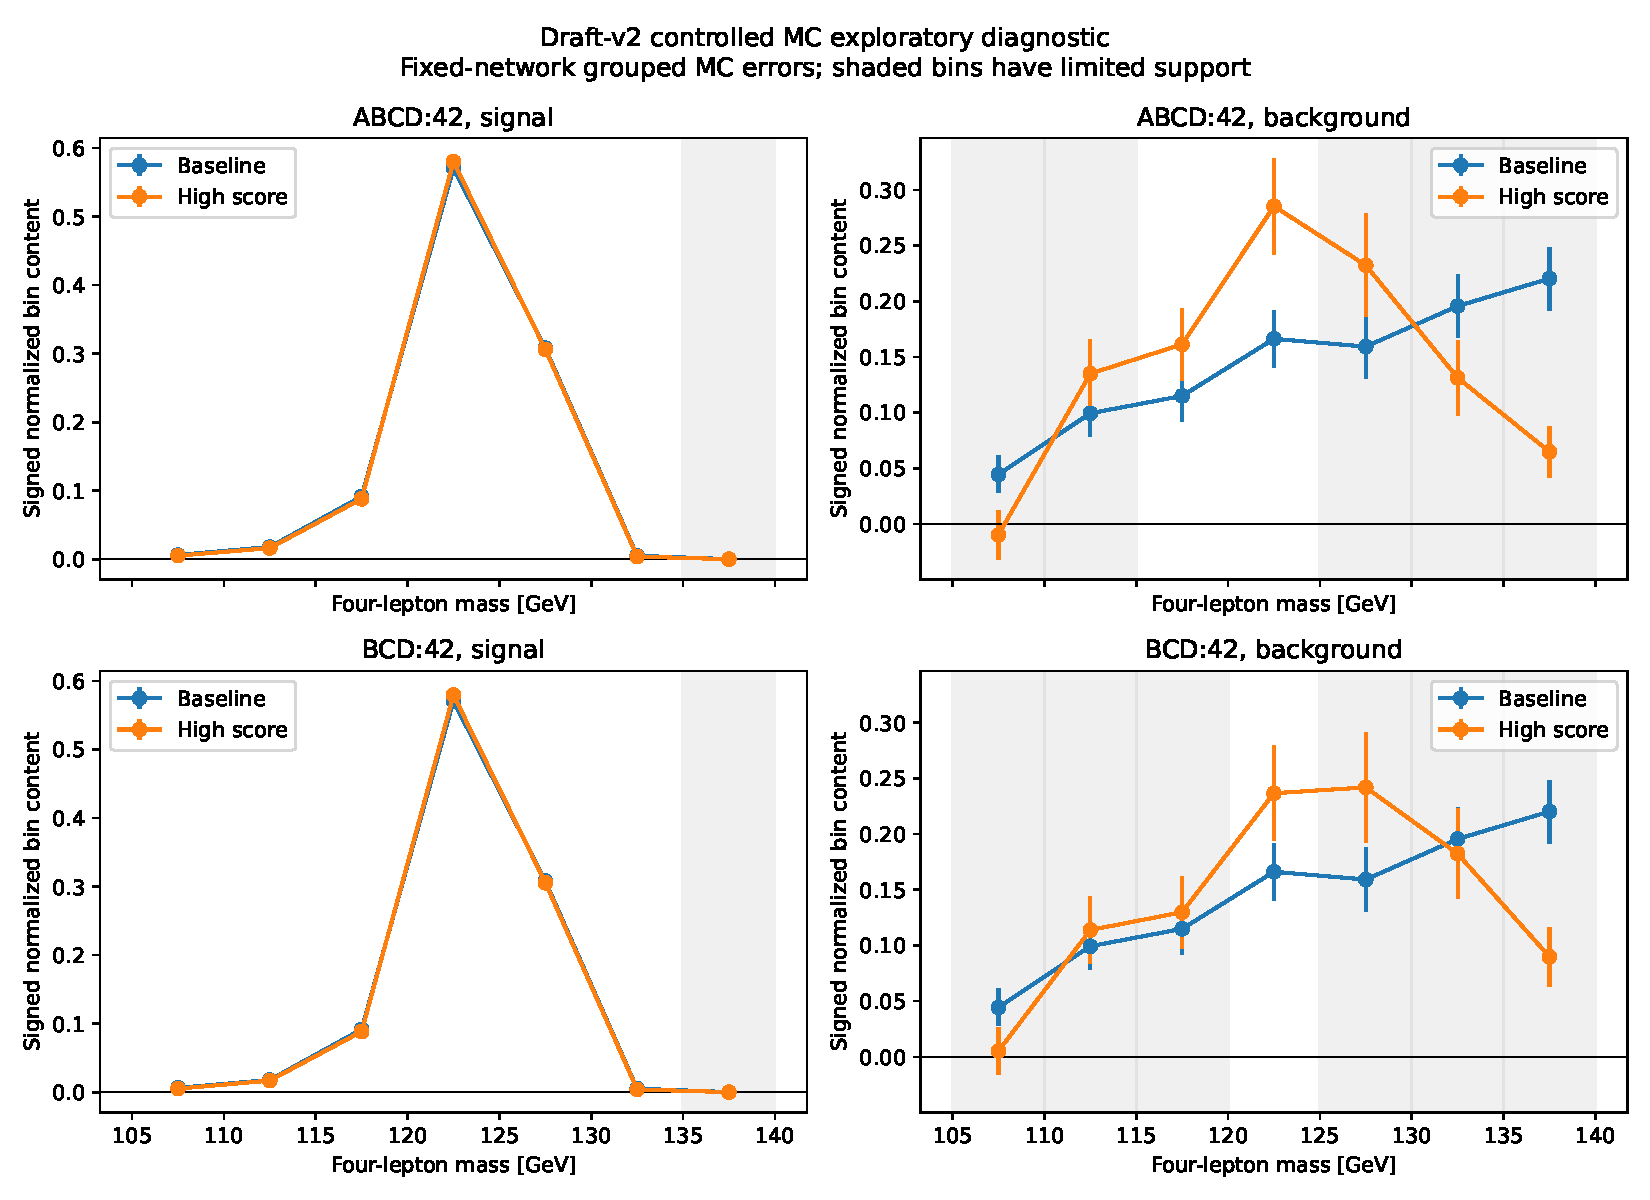
\includegraphics[width=.94\linewidth]{figures/draft001/mass-shapes.pdf}
\caption{与图~\ref{fig:yields} 使用相同事件和阈值、分别归一化后的筛选前后质量谱形。
每个箱除以其曲线自身为正的带符号总产额。误差传播包括共享归一化；筛选前后也共享事件。
带符号归一化谱形不一定是概率密度。保留阴影箱和负值箱，不作平滑、裁剪或重新分箱。}
\label{fig:shapes}
\end{figure}

\begin{table}[h!]
\caption{固定质量区域内的带符号产额占各自曲线总产额的比例（\%）。
数值为描述性点估计，未展示不确定度，不能据此判定筛选前后差异的统计显著性。}
\label{tab:fractions}
\centering
\small
\begin{tabular}{llrrr}
\toprule
过程 & 区域（GeV） & 筛选前 & ABCD 高分 & BCD 高分 \\
\midrule
信号 & $[120,130)$ & 87.9 & 88.6 & 88.5 \\
背景 & $[120,130)$ & 32.5 & 51.8 & 47.9 \\
背景 & $[135,140)$ & 22.0 & 6.5 & 9.0 \\
\bottomrule
\end{tabular}
\end{table}

\textbf{解释。} 信号仍集中于其主要质量区域；背景在该区域的相对占比上升，而高质量尾部占比下降。
这描述性地表明，即使不显式输入 $m_{4\ell}$，已冻结的选择仍与质量有关。
它不能确定唯一负责的输入特征，也不能证明背景存在物理共振。

\textbf{限制。} ABCD 筛选后的背景在 $[105,110)$ GeV 箱中为负；若干背景箱和信号高质量尾部的统计支持不足。
共享事件与归一化产生的相关性，使图中误差不能视为独立测量。误差以固定网络和阈值为条件，
不包含阈值估计、独立重训练及覆盖率不确定度。

\clearpage
\reportsection{7. 项目状态与下一步}
\textbf{已完成工作。} 简化研究已针对随机种子 42、43、44，分别训练 ABCD、BCD、ACD、ABD 和 ABC
五种表示。A/B/C/D 组依次描述单轻子运动学、双轻子质量与分离、事件整体运动学及五个角度。
每个删减输入模型均单独训练。全部 15 个标称区间及一个共享的包容计数参考均具有有效数值状态。

主要指标仍为 $W_{68}=\mu_{\rm upper}-\mu_{\rm lower}$，即指定模型下标称 68\% 信号强度区间的宽度。
信号强度 $\mu$ 缩放预期信号产额。每个区间采用其自身模型在注入 $\mu=1$ 时生成的 Asimov 期望观测，
由 T1 似然对有限模板统计的干扰参数作剖面化。在 $0\leq\mu\leq20$ 内，端点由剖面似然比统计量
达到一个自由度 $\chi^2$ 分布的渐近 68\% 分位数确定。标称 68\% 不代表重复抽样覆盖率已校准。
高分和低分两个类别均进入似然，各自在单一质量区间 $[105,140)$ GeV 上积分。
质量谱的七个展示箱不属于似然分箱；展示高分事件不意味着推断丢弃了低分事件。

\begin{table}[h!]
\caption{标称区间比较的进展摘要。中位数汇总三个固定训练种子，不代表重复的独立 MC 样本。}
\label{tab:widths}
\centering
\begin{tabular}{llr}
\toprule
输入表示 & 去掉的输入组 & $W_{68}$ 中位数 \\
\midrule
ABCD & 无 & 1.464392 \\
BCD & A & 1.474847 \\
ACD & B & 1.467509 \\
ABD & C & 1.505681 \\
ABC & D & 1.452977 \\
包容计数参考 & 不使用训练分类器 & 1.638845 \\
\bottomrule
\end{tabular}
\end{table}

四项比较先在每个种子内计算
$\Delta W_G=W_{68}(\mathrm{ABCD}\setminus G)-W_{68}(\mathrm{ABCD})$，再汇总。
去掉 C 使三个种子的区间均变宽，中位数为 $\Delta W_C=0.046283$。
A、B、D 的差值在不同种子间改变符号。ABC 在五种表示中的中位宽度最小，
但这不足以确立普遍最优的输入组合或已证实的精度提升。

\textbf{解释状态。} 这些结果属于探索性、非独立 MC 结果。重新划分后，研究仍使用先前已使用过的源事件。
区间以自身模板作为期望观测；覆盖率尚未独立校准。T1 在似然内处理有限模板统计，
但不提供不同模型区间宽度之差的完整 MC 不确定度。种子变化范围不是置信区间。
项目属于教育与技术研究，不是 ATLAS/CMS 官方结果、希格斯发现或物理测量。

\textbf{下一步。}
\begin{itemize}
\item 检查筛选前后比较是否充分解释了所选信号和背景。
\item 评估已记录的项目改动，并优先核实尚未确认的筛选条件来源。
\item 优先验证物理权重与筛选的适用性、宽度差的有限 MC 不确定度及区间覆盖率。这些工作仍待完成。
\end{itemize}

\clearpage
\reportsection{来源与简要溯源说明}
英文报告记录的外部来源核对日期为 2026 年 10 月 30 日。已发表分析提供筛选背景，
不提供本报告的数值结果。CERN 记录明确说明该数据集用于教育，不适用于科学出版。
本进展报告保持教育与技术研究范围；使用该数据集不意味着复现下列研究级分析。

\begingroup
\small
\renewcommand{\refname}{本报告参考文献}
\begin{thebibliography}{9}
\bibitem{OpenData}
ATLAS Collaboration, \emph{ATLAS 13 TeV samples collection at least four leptons
(electron or muon), for 2020 Open Data release} (2020).
\href{https://opendata.cern.ch/record/15005}{CERN Open Data record 15005},
\href{https://doi.org/10.7483/OPENDATA.ATLAS.2Y1T.TLGL}{doi:10.7483/OPENDATA.ATLAS.2Y1T.TLGL}.
两份模拟数据及发布前宽松预筛选说明的来源；使用限制见记录声明。

\bibitem{ATLAS13}
ATLAS Collaboration, \emph{Measurement of the Higgs boson coupling properties in
the $H\to ZZ^*\to4\ell$ decay channel at $\sqrt{s}=13$ TeV with the ATLAS detector},
JHEP \textbf{03} (2018) 095.
\href{https://doi.org/10.1007/JHEP03(2018)095}{doi:10.1007/JHEP03(2018)095};
\href{https://arxiv.org/pdf/1712.02304v2#page=8}{arXiv:1712.02304v2，第 5.1--5.2 节，第 8--9 页}。
本报告第 2--3 章筛选与工作点比较的来源。

\bibitem{HZZCuts}
ATLAS Open Data outreach tools, \emph{HZZCuts.py}，版本
\nolinkurl{8ad2015be6d350060c3a183aff5802570bc9ada4}。
\href{https://github.com/atlas-outreach-data-tools/atlas-outreach-Python-uproot-framework-13tev/blob/8ad2015be6d350060c3a183aff5802570bc9ada4/HZZCuts.py#L2-L33}{固定版本源码，第 2--33 行}。
多重数、电荷、部分动量条件、味道及可选隔离定义。

\bibitem{HZZAnalysis}
ATLAS Open Data outreach tools, \emph{HZZAnalysis.py}，版本同文献~\cite{HZZCuts}。
\href{https://github.com/atlas-outreach-data-tools/atlas-outreach-Python-uproot-framework-13tev/blob/8ad2015be6d350060c3a183aff5802570bc9ada4/HZZAnalysis.py#L140-L168}{固定版本源码，第 140--168 行}。
事件权重因子、实际施加的筛选及已注释的隔离调用。

\bibitem{ATLASRun1}
ATLAS Collaboration, \emph{Measurements of Higgs boson production and couplings
in the four-lepton channel in $pp$ collisions at center-of-mass energies of
7 and 8 TeV with the ATLAS detector}, Phys.~Rev.~D \textbf{91}, 012006 (2015).
\href{https://doi.org/10.1103/PhysRevD.91.012006}{doi:10.1103/PhysRevD.91.012006};
\href{https://arxiv.org/pdf/1408.5191v3#page=7}{arXiv:1408.5191v3，第 5.1 节，印刷页码第 6--7 页}。
触发匹配原则的参考；不声称其详细阈值和工作点与本项目相同。
\end{thebibliography}
\endgroup

\textbf{本地结果来源。} 区间、产额与质量谱结果及两幅图来自
\nolinkurl{runs/h4l-draft-v2-draft001/report/}，并关联已完成的准备、冻结和评估产物。
英文报告记录：报告文件大小与 SHA-256 已对照清单核对，两份图的副本与报告原图逐字节一致。
详细身份记录见 \nolinkurl{paper/draft-v2/DRAFT001-EVIDENCE.md}；
冻结协议为 \nolinkurl{config/protocols/h4l_draft_v2.json}。

\textbf{筛选实现。} 英文报告已对照 \nolinkurl{config/protocols/h4l_selection_v1.yaml}
及 \nolinkurl{src/higgsml/physics/selection.py} 核对精确不等式，并采用 draft-v2 协议的
$[105,140)$ GeV 质量窗口覆盖及 $2e2\mu$ 限制。本次修订依据 CERN 记录的方法说明，以及已完成运行的协议、模型元数据和汇总结果。
表~\ref{tab:population} 的输入数来自绑定的数据集记录，筛选后及分配数来自 prepare 文件的身份外壳计数，
并核对该文件的清单哈希；未解码事件数值载荷。网络结构和阈值算法另对照
\nolinkurl{src/higgsml/draft_v2/training.py} 及
\nolinkurl{src/higgsml/modeling/discriminants.py} 核实，模型文件与其清单哈希一致。
未重新训练、计算事件分数或拟合区间。逐条筛选计数仍未提供，不用其他运行结果估算。

\end{document}
